%%
%% Template conclusion.tex
%%

\chapter{Results}
\label{cha:Results}
In this chapter, we provided our experiment results using different methods and data sets. We started by a brief analysis of our data set. Then we discussed and compared the results of various methods, including convolutional neural networks, ZCA whitening, convolutional auto-encoders, super-pixel labeling and super-pixel denoising, respectively. Thereafter, we evaluated their performance on manually annotated data. 

\section{Data Set Attributes}
Our training set contained 264 road scene images and generated labels, which had been rescaled to the resolution of 128 by 348 pixels. We chose a patch size of 32 by 32, which we believed to be an appropriate size that can reflect the local property around a pixel and at same time contain sufficient information for inferring which category it belongs to. 

The distribution of pixels with respect to each category was unbalanced. Since we used the softmax error function, different cases of misclassification were equally weighted. Therefore an unbalanced data set was going to bias the classification result to be in favor of the category of the largest population.
\section{Convolutional Neural Networks}
\label{Baseline}
\subsection{Training and test set}
In order to build a balanced training set, for each image, we randomly selected 25 pixels from each category, and extracted their surrounding patches (of size 32 by 32) accordingly. A number of 75 ($25\times3$) patches selected from a 128 by 348 image will roughly cover every part of the image. In total our training set consisted of $3\times25\times264 = 19,800$ patches evenly taken from each category, which will be referred to as \textit{gen\_train} set in following discussions. 

We have 205 separate images available for testing, the \textit{patch\_test} set was extracted by randomly selecting 100 patches from each image in the test set. Thus \textit{patch\_test} set was an unbalanced set consisted of $100\times205 = 20,500$ patches.
\subsection{Outcome}
We trained a convolutional neural network directly on the \textit{gen\_train} set using stochastic gradient decent for 100 epochs, and then tested it against the \textit{patch\_test} set. The training error was $0.1535$, the test error was $0.1974$. This result was used as a baseline for evaluating the effectiveness of other methods. An example prediction outcome is shown in Figure \ref{cnnpredfig}.

\begin{figure}[h!]
\centering
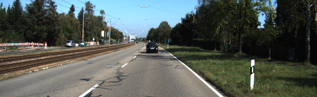
\includegraphics[width=0.7\linewidth]{pics/img.png}

\includegraphics[width=0.7\linewidth]{pics/cae.png}
\caption{The prediction result (bottom) using convolutional neutral network train on \textit{gen\_train} set of a input image (top).}
\label{cnnpredfig}
\end{figure}

The convolutional neural network we used was composed of 4 layers, the first layer was a convolutional layer using 5 by 5 kernels and 15 feature maps, the second layer was a max pooling layer using 2 by 2 pools, the third layer was similar to the first using 24 feature maps instead, the four layer was the same as the second. How we chose thees architectural parameters will be discussed in Section \ref{sec: cae}.

\section{ZCA Whitening}
\subsection{Pre-training data set}
When applying ZCA whitening in the pre-processing step, we need to do the same pre-processing operation for the test data because our classifier would then be trained on whitened images. From Equations \ref{pcaeq1} and \ref{pcaeq2} we can infer that the bases of the projective space $U$ should be independent of how the data were drawn from the ensemble of all the road scene images. Thus for a better generalizability on unknown data, it would be more reasonable if we apply a more general data set to estimate the projective space $U$.

Therefore out data for pre-processing were drawn from a larger set of 942 images, which is a combination of our training set and other road scene images from the KITTI data set. More specifically, we took 32 patches from each image so that in total $30,144$ patches was contained. This set will be denoted as the \textit{pre\_train} set in the following sections.
\subsection{Outcome}
We evaluated the parameters for ZCA whitening on the \textit{pre\_train} set, and trained the convolutional neural networks in the same manner as described in Section \ref{Baseline}. The training error was $0.1245$, the test error was $0.1786$, which shows an improvement of $1.9\%$ than the baseline. An example outcome using ZCA whitening is shown in Figure \ref{cnnpredfig}.

\begin{figure}[h!]
\centering
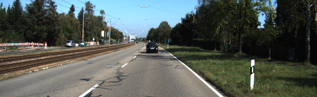
\includegraphics[width=0.7\linewidth]{pics/img.png}

\includegraphics[width=0.7\linewidth]{pics/raw.png}
\caption{The prediction result (bottom) using ZCA whitening of the same input image (top). It shows some improvement compared to Figure \ref{cnnpredfig}.}
\label{zcapredfig}
\end{figure}

\section{Convolutional Auto-encoders}
\label{sec: cae}
\subsection{Unsupervised feature learning}
Convolutional auto-encoders is an unsupervised learning approach. For similar reasons as ZCA whitening, we experimented the convolutional auto-encoders over the \textit{pre\_train} set for better generalizability. Following the same fashion as described in Section \ref{sec:Unsupervised Feature Learning}, the fist layer reconstruction error tended to converge at 15 feature maps with 5 by 5 kernel size, the second layer reconstruction error tended to converge at 24 feature maps with 5 by 5 kernel size. The reconstruction error (\ref{aeerr}) of 32 by 32 RGB patches converged at around 13.3 in our experiment. Visualization of selected first layer kernels are shown in Figure \ref{kernelfig}.

\begin{figure}[h!]
  \centering  
  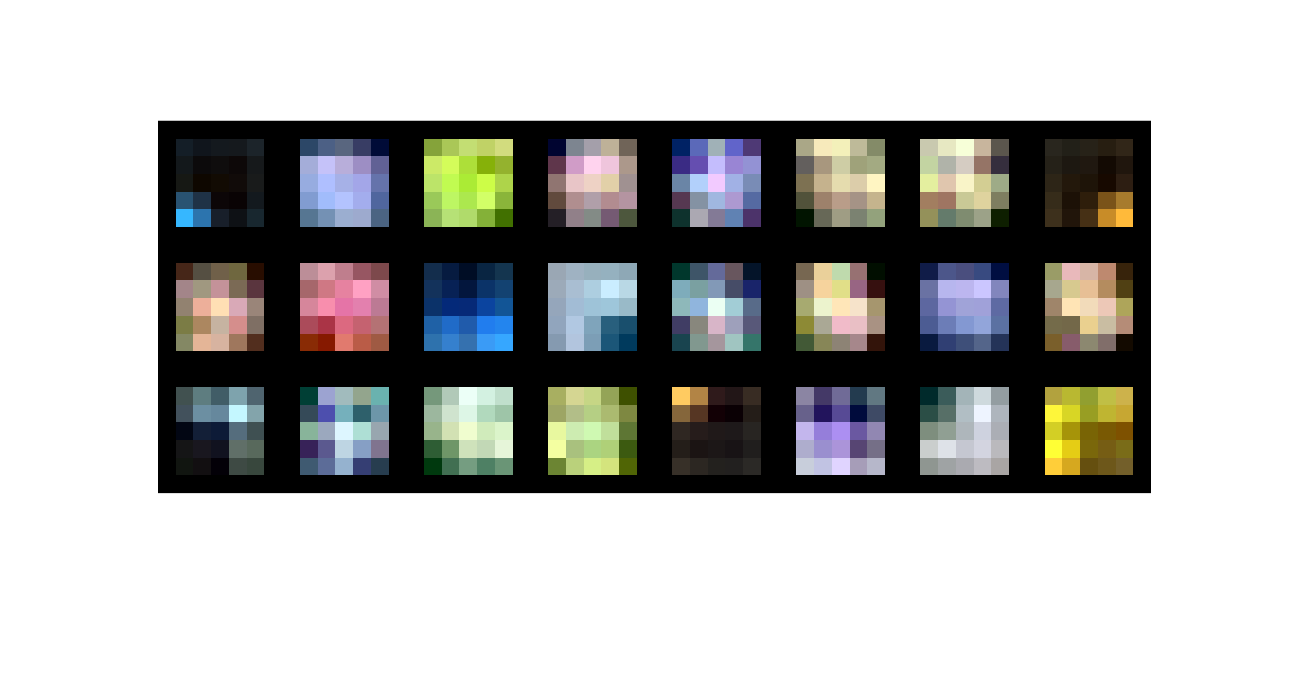
\includegraphics[width=0.8\textwidth]{pics/kernels.png}
  \caption{A number of 24 first layer kernels trained on the \textit{pre\_train set} set. As we can see some of the feature do not have an obvious pattern, in fact they are associated with much lower weights.}
  \label{kernelfig}
\end{figure}

An interesting observation was if we apply a more complected architecture, such as increasing the number of feature maps, we are likely to have more lightweight features with no obvious patterns or heavyweight features similar to existing ones. Which again confirmed our belief that the network architecture we adopted was reasonable.

\subsection{Outcome}
After we applied the parameters of a trained convolutional auto-encoder directly as the initialization of a corresponding convolutional neural network, trained and tested in the same manner in Section \ref{Baseline}, we obtained a training error of $0.1237$, and a test error of $0.1726$, which shows an improvement of $0.6\%$ than using ZCA whitening and $2.5\%$ than the baseline. Moreover, the number of epochs required for training error to converge had decreased as the convolutional neural network was well initialized .

\section{Super-pixel Labeling}

For super-pixel labeling (Section \ref{sec:Super-pixel labeling}), we segmented each image into approximately 300 super-pixels, which turned out to be a relatively small number but sufficient to capture the outline of the image. The 205 images in the test set are used directly, and will be referred to as \textit{super\_test} set. As was shown in Table \ref{supertab}, when super-pixel labeling was applied, the outcomes of the above three learning methods were improved by different percentages ranging from $0.24\%$ to $0.56\%$. A sample outcome of super-pixel labeling is shown in Figure \ref{superpredfig}.

\begin{table}
	\centering	
	\begin{tabular}{lcc}	
				& \textit{patch\_test} & \textit{super\_test}\\
	\hline
	Raw 			& 0.1974	 & 0.1918\\
	ZCA			& 0.1786	 & 0.1762\\
	CAE			& 0.1726 & 0.1701\\	
	\end{tabular}	
	\caption{Test error of different learning and testing methods.  Rows indicate learning methods, Raw denotes using raw data as input, ZCA denotes using ZCA whitening to pre-process, CAE stands for using a trained convolutional auto-encoder to initialize. Columns indicate test methods and test sets explained previously.}
	\label{supertab}	
\end{table}

\begin{figure}[h!]
\centering
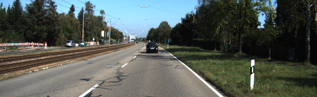
\includegraphics[width=0.7\linewidth]{pics/img.png}

\includegraphics[width=0.7\linewidth]{pics/super.png}
\caption{The prediction result (bottom) using convolutional auto-encoders and super-pixel denoising. It again shows some improvement compared to Figure \ref{cnnpredfig} and \ref{zcapredfig}.}
\label{superpredfig}
\end{figure}

\section{Super-pixel Denoising} 
As we can see from Figure \ref{superpredfig}, the super-pixel labeling output could be noisy. After MRF denoising, the labels became much smoother (Figure \ref{mrfpredfig}). However, it also changed some correctly classified but isolated super-pixels in to other categories, in order to achieve a smooth picture. Moreover, because its effectiveness depends on how the misclassifications were distributed, it in fact could decrease the accuracy in many other cases.

\begin{figure}[h!]
\centering

\includegraphics[width=0.7\linewidth]{pics/super.png}

\includegraphics[width=0.7\linewidth]{pics/denoise.png}
\caption{The denoised result using Markov random fields. Tough the image has become much smoother, some correctly labeled areas were regarded as noise (e.g., sky in the top left region).}
\label{mrfpredfig}
\end{figure}

\section{Manual Labels}
\subsection{Manual training and test sets}
The noticeable amount of noise in generated labels brings uncertainty of the validity of our test results. Therefore we used 20 manually labeled images from separate scenarios (referred to as \textit{manual\_test} set) to explore the real world applicability of our system.

To further investigate the influence of noisy training data, we repeated out experiments on another set of training data (\textit{manual\_train} set), which consisted of 25 patches randomly selected from each category of 40 manually labeled images. Only \textit{manual\_test} set was used for test here, since it would be meaningless to test on noisy labels.

\subsection{Outcome}
\begin{figure}[h!]
\centering
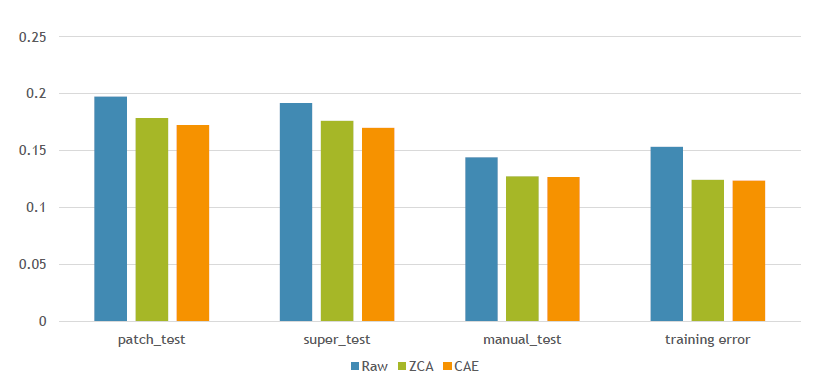
\includegraphics[width=\linewidth]{pics/res.png}
\caption{Training and test error of different approaches (denoted by columns) on different test sets or test methods (denoted by colours). The smallest error on noiseless test data (orange bar in the third column) was acquired by the combination of convolutional auto-encoders and super-pixel labeling.}
\label{resfig}
\end{figure}

As was shown in the figure \ref{resfig}, all these methods had substantive increases (around $5\%$) in accuracy when tested on noise free data. If in the cases where ZCA whitening and convolutional auto-encoders are used, we achieved around $12.7\%$ error rate, which is almost the same as the noise ratio we have in the training data.

\begin{table}[h!]
	\centering		
	\begin{tabular}{lcc}	
				& \textit{gen\_train} set & \textit{manual\_train} set\\
	\hline
	Raw 			& 0.1442 & 0.1320 \\
	ZCA			& 0.1274 & 0.1173 \\
	CAE			& 0.1267 & 0.1049 \\	
	\end{tabular}	
	\caption{Test error of different training sets on \textit{super\_test} set using super-pixel labeling.}
	\label{mantab}
\end{table}

Comparing Table \ref{mantab} with Table \ref{supertab} we can see, although only a small amount of training data was engaged, the test result on manual labels shows an improvement of $1\%$ to $2\%$.

%%% Local Variables: 
%%% mode: latex
%%% TeX-master: "thesis"
%%% End: 
